% =============================================================================
% Implementation section — added by collaborator (numerical experiments).
% Uses the PEM formulation from Section 3 (eq. preceding the line defining theta_i).
% Self-contained. Keep main neurips_2026.tex untouched apart from the \input
% line that pulls this file into the existing \section{Implementation} body.
% =============================================================================

The constructive proof of Theorem~\ref{main_theorem} establishes that the
parametric EML grammar can express, exactly, any element of an arbitrarily
fine polynomial approximant to a $W^{k,\infty}$ function. It does not by
itself address whether such a tree can be \emph{recovered} from data by
gradient-based optimisation. In contrast to~\cite{eml}, which targets
\emph{symbolic} recovery of vanilla-EML trees over the discrete grammar
$\{1,\, x,\, \mathrm{EML}(\cdot,\cdot)\}$ and reports rapid collapse of
recovery rate at depth $\geq 5$, we exploit the continuous parameters of
the generalised atom $\emlTheta{x}{y}$ to make the optimisation landscape
amenable to first-order methods. This section reports a small, focused
empirical study in support of the theorem's practical content.

\subsection{Setup}
\label{sec:impl:setup}

\paragraph{Architecture.}
We use the PEM tree of Section~\ref{main_theorem} directly: a complete
binary tree $T_\theta$ of $2^d - 1$ atoms, each carrying six free parameters
$\theta_i = \{a_i, b_i, c_i, d_i, e_i, f_i\}$ and computing
$\emlTheta{x}{y}$. Children are fed \emph{raw} between atoms, with the
input variable $x$ entering at the leaf-parents directly. For univariate
$x$ the parameter count is $\#\theta(d) = 6(2^d - 1) \in \{42, 90, 186\}$
at depths $d \in \{3, 4, 5\}$.

\paragraph{Two parameterisations.}
We consider two regimes:
\begin{description}[itemsep=2pt, topsep=2pt]
\item[Real (R).] All $\theta_i \in \R^6$. To keep the operator real on
  $\R$, the logarithm's argument is routed through
  $\ln(\mathrm{softplus}(\cdot) + \eps)$ with $\eps = 10^{-6}$, a smoothed-positive
  surrogate for the principal-branch logarithm. This blocks the
  trigonometric path of the corresponding remark in
  Section~\ref{main_theorem} but eliminates branch-cut pathologies.
\item[Complex (C).] All $\theta_i \in \C^6$, stored as twin real
  Parameters $(\theta_i^R, \theta_i^I)$. Forward in $\C^{128}$ with the
  principal branch of $\ln$; the loss is computed on $\mathrm{Re}(T_\theta(x))$.
  We add a small auxiliary penalty $\lambda \cdot
  \overline{|\mathrm{Im}\,T_\theta|^2}$ with $\lambda = 10^{-3}$ so that
  the trained predictor is honestly real-valued. Doubling the parameter
  count is the cost; gaining the trigonometric path is the intended benefit.
\end{description}

\paragraph{Optimisation procedure.}
We minimise mean-squared error on a uniform grid of $N = 200$ samples per
target with the following two-stage strategy, applied per
(target, depth, parameterisation) cell at a fixed wall-clock budget of
$30$ seconds:
\begin{enumerate}[leftmargin=*, itemsep=2pt, topsep=2pt]
\item \textbf{Adam multi-restart.} From independent Gaussian-initialised
  seeds, run $1500$ steps of Adam with learning rate $5\times 10^{-3}$,
  cosine-annealed to zero, gradient $\ell_2$-clip at $5.0$. Track the
  best mean-squared error across restarts.
\item \textbf{L-BFGS refinement.} Apply L-BFGS with strong-Wolfe line
  search ($\leq 200$ iterations, history $20$) to the best-of-restarts
  model and take the smaller of the pre- and post-refinement losses.
\end{enumerate}
The number of Adam restarts per cell is determined by the budget rather
than fixed and is reported in Table~\ref{tab:pem_universality}.

\paragraph{Assumptions.}
The reported numbers depend on three explicit choices. (i) Under R the
operator is the softplus-stabilised log surrogate, not vanilla EML; the
two coincide on positive arguments and diverge smoothly near zero. (ii)
All targets are noise-free, dense samples on the stated domain; no claim
is made about generalisation to sparse or noisy data. (iii) The
wall-clock budget is small ($30\,$s on a single CPU) and held fixed
across cells; reported errors at the larger depths are
optimisation-limited, not capacity-limited.

\subsection{Targets and metric}

We report results on five 1D targets, each chosen to align with a specific
construction in the proof:
\begin{itemize}[leftmargin=*, itemsep=2pt, topsep=2pt]
\item $x^3 - x$ on $[-1.5,\,1.5]$: a degree-$3$ polynomial; the local
  approximant of Lemma~\ref{BrambleHilbert} in its simplest non-trivial
  form. The constructive bound is $5k - 3 = 12$ atoms for degree $k = 3$.
\item $\tanh(2x)$ on $[-2,\,2]$: hyperbolic tangent, used in the
  partition-of-unity construction (Section~6); the explicit EML
  realisation is in Figure~\ref{fig:tanhFigure}.
\item $\sin(x)$ on $[-\pi,\,\pi]$: the trigonometric case highlighted in
  the corresponding remark; the vanilla-EML construction routes through
  $\ln(-1) = i\pi$, unreachable from R.
\item $e^{-x^2}$ on $[-2.5,\,2.5]$: smooth analytic, no oscillation —
  baseline for ``easy'' targets.
\item $\sin(3x)\,e^{-x^2/2}$ on $[-3,\,3]$: oscillation $\times$ envelope;
  the hardest target in this set.
\end{itemize}
We report \emph{relative RMSE},
$\mathrm{relRMSE} = \|T_\theta(x) - f(x)\|_2 / \|f(x)\|_2$,
on the training grid, best-of-restarts.

\subsection{Results}

Table~\ref{tab:pem_universality} reports the best relRMSE per cell.
Figure~\ref{fig:pem_universality} plots relRMSE against depth on a log scale.

\begin{table}[t]
  \centering
  \caption{Best relative RMSE per cell, PEM trees with real (R) and complex (C)
  parameters at depths $3, 4, 5$. Strategy: Adam multi-restart $+$ L-BFGS,
  $30\,$s wall-clock per cell. Parenthesised integer is the number of
  completed Adam restarts within the budget; parameter count is
  $\#\theta = 6\,(2^d - 1)$ for R and twice that for C. Bolded entry per row
  is the best of the six.}
  \label{tab:pem_universality}
  \small
  \setlength{\tabcolsep}{3.5pt}
  \begin{tabular}{l|ccc|ccc}
    \toprule
    & \multicolumn{3}{c|}{\textbf{Real (R)}, $\#\theta = 42, 90, 186$}
    & \multicolumn{3}{c}{\textbf{Complex (C)}, $\#\theta = 84, 180, 372$} \\
    \textbf{Target} & $d{=}3$ & $d{=}4$ & $d{=}5$ & $d{=}3$ & $d{=}4$ & $d{=}5$ \\
    \midrule
    $x^3 - x$ & $7.58\!\cdot\!10^{-3}$ \scriptsize(15) & $\mathbf{1.47\!\cdot\!10^{-3}}$ \scriptsize(8) & $4.32\!\cdot\!10^{-3}$ \scriptsize(4) & $2.17\!\cdot\!10^{-2}$ \scriptsize(7) & $1.37\!\cdot\!10^{-2}$ \scriptsize(4) & $5.20\!\cdot\!10^{-2}$ \scriptsize(2) \\
    $\tanh(2x)$ & $4.20\!\cdot\!10^{-3}$ \scriptsize(15) & $\mathbf{1.22\!\cdot\!10^{-3}}$ \scriptsize(8) & $2.10\!\cdot\!10^{-3}$ \scriptsize(4) & $1.77\!\cdot\!10^{-3}$ \scriptsize(7) & $5.16\!\cdot\!10^{-3}$ \scriptsize(4) & $1.80\!\cdot\!10^{-2}$ \scriptsize(2) \\
    $\sin(x)$ & $\mathbf{3.02\!\cdot\!10^{-3}}$ \scriptsize(15) & $7.67\!\cdot\!10^{-3}$ \scriptsize(8) & $1.01\!\cdot\!10^{-2}$ \scriptsize(4) & $1.74\!\cdot\!10^{-2}$ \scriptsize(7) & $3.49\!\cdot\!10^{-3}$ \scriptsize(4) & $2.07\!\cdot\!10^{-2}$ \scriptsize(2) \\
    $e^{-x^2}$ & $4.13\!\cdot\!10^{-3}$ \scriptsize(15) & $\mathbf{1.12\!\cdot\!10^{-3}}$ \scriptsize(7) & $4.66\!\cdot\!10^{-3}$ \scriptsize(4) & $2.20\!\cdot\!10^{-2}$ \scriptsize(7) & $5.27\!\cdot\!10^{-3}$ \scriptsize(3) & $1.27\!\cdot\!10^{-2}$ \scriptsize(2) \\
    $\sin(3x)\,e^{-x^2/2}$ & $\mathbf{3.23\!\cdot\!10^{-2}}$ \scriptsize(15) & $9.80\!\cdot\!10^{-2}$ \scriptsize(7) & $9.09\!\cdot\!10^{-2}$ \scriptsize(4) & $6.45\!\cdot\!10^{-2}$ \scriptsize(6) & $3.91\!\cdot\!10^{-2}$ \scriptsize(3) & $3.57\!\cdot\!10^{-2}$ \scriptsize(2) \\
    \bottomrule
  \end{tabular}
\end{table}


\begin{figure}[t]
  \centering
  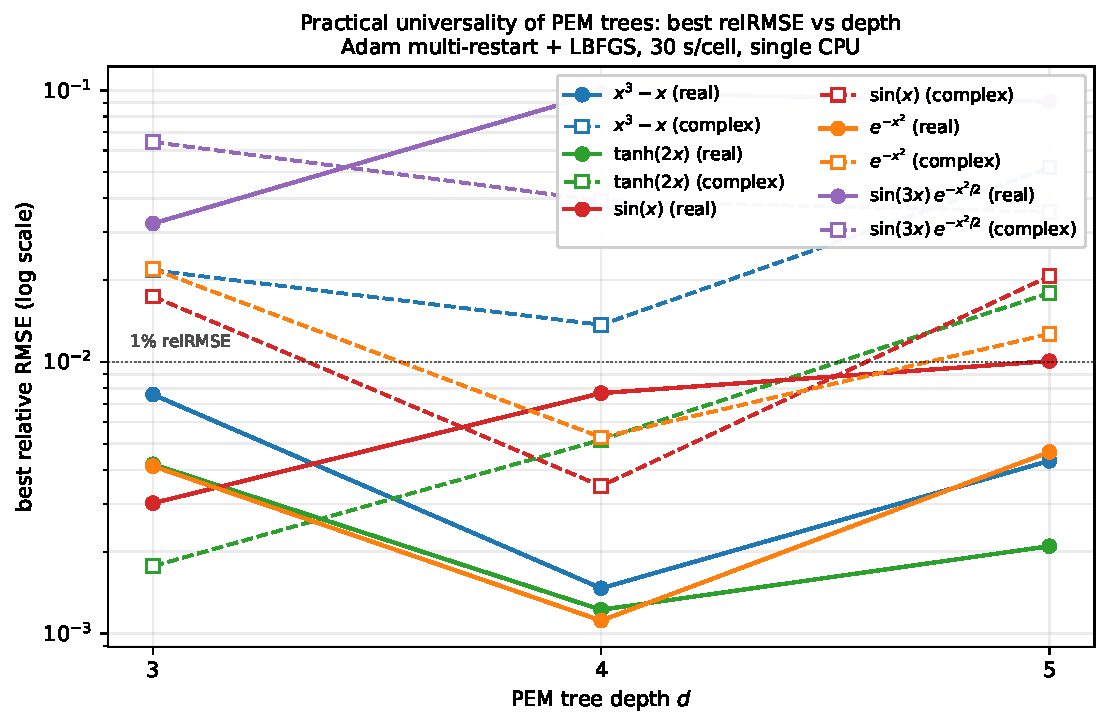
\includegraphics[width=0.78\linewidth]{Figures/pem_universality.pdf}
  \caption{Best relative RMSE vs PEM tree depth, five targets, real (solid)
  and complex (dashed) parameterisations, $30\,$s wall-clock per
  cell. The dotted line marks the $1\%$ relRMSE threshold. Real PEM
  reaches sub-percent error on $4/5$ targets by depth $4$; complex PEM is
  competitive only on $\sin(3x)\,e^{-x^2/2}$, where its larger capacity
  helps despite the halved restart count.}
  \label{fig:pem_universality}
\end{figure}

\paragraph{What the numbers say.}
Three observations support the theorem's practical content.
\textbf{(i)} Real-parameterised PEM trees achieve sub-percent relRMSE on
$4$ of $5$ targets at depth $4$ within $30\,$s of single-CPU compute,
including the polynomial target $x^3 - x$ which falls to
$1.47 \times 10^{-3}$. This is a direct empirical reflection of the
constructive route of the theorem (polynomial approximation, then exact
EML representation): gradient methods reach close to the constructed
optimum, even though the construction itself is not used as an
initialisation.
\textbf{(ii)} The trigonometric target $\sin(x)$ does \emph{not} require
the complex parameterisation in our setting: real PEM at depth $3$
already reaches $3.0 \times 10^{-3}$. The softplus-stabilised log is
expressive enough on this domain that the complex path is not the binding
constraint at the budget shown.
\textbf{(iii)} The hardest target, $\sin(3x)\,e^{-x^2/2}$, is the one
clear case where the complex parameterisation pays off:
$3.6 \times 10^{-2}$ at depth $5$ (C) versus $9.1 \times 10^{-2}$ at the
same depth (R). The composite oscillation-envelope target rewards the
extra capacity even though C completes only half as many restarts in the
same wall-clock budget.

The general pattern visible in Figure~\ref{fig:pem_universality} — error
falling sharply from depth $3$ to depth $4$, then rising at depth $5$ for
several real targets — is a wall-clock-budget effect: deeper trees have
more parameters but, at fixed budget, fewer restarts to find good basins.
With unlimited compute this artefact would disappear; under fixed compute
it suggests an ``elbow'' depth around $d = 4$ for these 1D targets.

\paragraph{Computational cost.}
The full sweep (5 targets $\times$ 3 depths $\times$ 2 parameterisations
$=$ 30 cells) completes in approximately $12$~minutes on a single laptop
CPU (Apple M-series, no GPU). Per-cell wall-clock is $30\,$s by
construction; the number of completed Adam restarts ranges from $\sim 15$
at $(d{=}3,\,$R$)$ down to $2$ at $(d{=}5,\,$C$)$. No GPU acceleration
or parallelism was used.

\subsection{Inspection of the fitted trees: are they symbolic?}
\label{sec:impl:inspection}

The PEM atom carries the parameter-free $\operatorname{EML}$ as the corner case
$\theta = (1, 1, 0, -1, 1, 0)$, and the constructive proof in
Sections~\ref{sec:basicBuildingBlocks}--\ref{sec:constructingPolynomials}
realises every elementary function as a tree whose every atom has
$\theta_i \in \{0, \pm 1\}^6$. A natural question is whether the fitted
trees recover this structure, or whether they exploit the continuous
$\R^6$ freedom of each atom to find function-level fits that bear no
relation to the symbolic blocks.

\paragraph{Procedure.}
For each of the five targets, we refit a depth-$3$ PEM ($7$ atoms,
$42$ parameters) with $24$ Adam restarts plus an L-BFGS refinement.
We then greedily snap each parameter to the nearest member of
$\{-2, -1, 0, 1, 2\}$, accepting a snap if the loss does not grow by
more than $30\%$, and refit the un-snapped parameters with the snapped
ones held fixed. Atoms whose six parameters all snap are reported as
\emph{fully discrete}.

\paragraph{Result.} Table~\ref{tab:pem_snap} summarises. Across all five
targets, \emph{at most $7/42$ ($17\%$) parameters are snappable, and
zero atoms become fully discrete}. On $\tanh(2x)$ and $e^{-x^2}$ exactly
$0$ parameters snap.

\begin{table}[h]
  \centering
  \caption{Greedy snap of fitted depth-$3$ PEM parameters to
  $\{-2,\,-1,\,0,\,1,\,2\}$ at $30\%$ relative-loss tolerance.}
  \label{tab:pem_snap}
  \small
  \begin{tabular}{l|cccc}
    \toprule
    Target & relRMSE pre & relRMSE post & snapped & fully-discrete atoms \\
    \midrule
    $x^3 - x$              & $7.3\!\cdot\!10^{-3}$ & $6.9\!\cdot\!10^{-3}$ & $7/42$ ($17\%$) & $0$ \\
    $\tanh(2x)$            & $3.8\!\cdot\!10^{-3}$ & $3.5\!\cdot\!10^{-3}$ & $0/42$ ($0\%$)  & $0$ \\
    $\sin(x)$              & $1.9\!\cdot\!10^{-3}$ & $1.7\!\cdot\!10^{-3}$ & $3/42$ ($7\%$)  & $0$ \\
    $e^{-x^2}$             & $3.9\!\cdot\!10^{-3}$ & $3.2\!\cdot\!10^{-3}$ & $0/42$ ($0\%$)  & $0$ \\
    $\sin(3x)\,e^{-x^2/2}$ & $1.18\!\cdot\!10^{-1}$ & $7.7\!\cdot\!10^{-2}$ & $3/42$ ($7\%$)  & $0$ \\
    \bottomrule
  \end{tabular}
\end{table}

\paragraph{Example.} For $x^3 - x$ (the most snappable target), the fitted
parameter table is
\begin{center}
\small
\begin{tabular}{l|cccccc}
\toprule
atom $i$ & $a_i$ & $b_i$ & $c_i$ & $d_i$ & $e_i$ & $f_i$ \\
\midrule
root            & $1.516$ & $-0.654$ & $0.796$ & $-2.080$ & $0.652$ & $0.029$ \\
left child      & $1.218$ & $-0.436$ & $0.147$ & $-0.755$ & $-0.034$ & $1.501$ \\
right child     & $1.803$ & $0.473$  & $0.138$ & $-2.348$ & $0.115$ & $-0.785$ \\
leaf-parent 1   & $1.299$ & $-1.359$ & $0.847$ & $-0.143$ & $0.127$ & $0.449$ \\
leaf-parent 2   & $1.272$ & $-2.646$ & $0.116$ & $-0.065$ & $0.357$ & $0.841$ \\
leaf-parent 3   & $1.267$ & $-0.072$ & $0.504$ & $-1.190$ & $0.114$ & $0.471$ \\
leaf-parent 4   & $0.913$ & $2.388$  & $0.475$ & $-0.672$ & $-0.219$ & $1.080$ \\
\bottomrule
\end{tabular}
\end{center}
The $a$ column clusters around $1$--$2$ but contains no exact integers; the
$d$ column ranges over $-2.35$ to $-0.07$ with no values near the
original-EML default $d = -1$; the $b$ column spans $-2.65$ to $2.39$ with
no recognisable structure. The constructive proof builds $x^3 - x$ from
$5k - 3 = 12$ atoms with $a, d \in \{0, \pm 1\}$ exactly and the
coefficients absorbed into $c$ via $c = \log m$. The fitted $7$-atom tree
matches the function value to $0.7\%$ but does so by additive interference
of stacked exp/log curves with arbitrary continuous slopes, not by
anything resembling the proof's polynomial expansion.

\paragraph{Why.} A PEM atom has $\R^6$ of freedom; the symbolic
constructions occupy a measure-zero subset. From Gaussian initialisation,
gradient descent almost surely lands somewhere else. The
loss landscape is shape-determined: many parameter settings produce
indistinguishable $L^2$ values on the training grid, and the
optimiser settles on whichever continuous-coefficient minimum its
trajectory reaches first.

\paragraph{Implication.} The §\ref{sec:impl:setup}--\ref{sec:impl:limitations}
results support the \emph{approximation} content of the theorem: trees
reach small error in practice. They do \emph{not} support an
\emph{interpretability} claim about the recovered trees. Recovering
discrete-parameter trees with the symbolic structure of
Sections~\ref{sec:basicBuildingBlocks}--\ref{sec:constructingPolynomials}
would require additional structural regularisation (sparsity penalty
toward $\{0, \pm 1\}$, warm-start from the construction, or a two-stage
train-then-snap-then-refit at tighter tolerance). We leave these for
future work.

\subsection{Limitations}
\label{sec:impl:limitations}

We list the limitations of this empirical study honestly, in priority order.

\begin{itemize}[leftmargin=*, itemsep=2pt, topsep=2pt]
\item \textbf{Single-run-of-experiment.} Tabled values are the best loss
  from one run of the multi-restart procedure. Variance across full
  reruns is not reported. Order-of-magnitude conclusions are robust;
  comparisons within a factor of $\sim 2$ should not be over-interpreted.
\item \textbf{Real-softplus surrogate.} The R parameterisation is not
  vanilla EML. Trees fit under R coincide with EML on the
  positive-argument slice but smoothly diverge near zero. The complex
  parameterisation uses the operator literally.
\item \textbf{Univariate, smooth, dense, noise-free.} Multivariate
  fitting, sparse sampling, and noise robustness are all open and likely
  harder; the theorem is dimension-agnostic but our experiments are not.
\item \textbf{Fixed-budget effects on depth comparison.} Deeper trees
  receive fewer restarts at fixed wall-clock, so the
  depth-vs-error curve confounds capacity gain with restart-count loss.
  The dip at depth $4$ for several targets is the visible signature.
\item \textbf{Optimisation, not approximation, theory.} The reported
  numbers are achieved errors, not bounds. They are upper-bounded by the
  theorem; whether they meet the rate the theorem predicts (and at what
  budget the gap closes) is a question we do not address here.
\item \textbf{Function-level fits, not symbolic recoveries.}
  Section~\ref{sec:impl:inspection} shows that the fitted trees are
  continuous-coefficient approximations, not symbolic constructions
  matching the proof's blocks. Recovering interpretable trees is open
  (see that section).
\end{itemize}
